\section{Transformation des Ereignisverarbeitungsdienstesin ausführbaren Code}\label{sec:Transformation}

Der Ereignisverarbeitungsdienst wird im Rahmen der Bachelorarbeit als Webservice auf der SAP Cloud Platform entwickelt. Die verwendeten Frameworks werden im Folgenden kurz beschrieben:

\paragraph{Java} Die SAP Cloud Platform erlaubt mit Java als Programmiersprache, moderne \ac{SOA}-orientierte Webservices zu entwickeln. Die SAP Cloud Platform unterstützt dabei, Java-Anwendungen in einer Cloud-Umgebung zu bauen, zu deployen und zu betreiben. Als Laufzeitumgebung steht dabei Java Platform, Enterprise Edition (Java EE) mit einer großen Auswahl an APIs und einem einfachen Programmiermodell zur Verfügung. \cite{Schneider.2018}

\paragraph{Spring Framework} Die softwaretechnische Implementierung erfolgt durch das Spring Framework. Das Spring Framework bietet ein umfassendes Programmier- und Konfigurationsmodell für moderne Java-basierte Anwendungssoftware. Das Framework ist sehr verbreitet bei der Entwicklung von Webservcie.
\cite{Herzig.2018}

\paragraph{SAP Cloud Platform SDK for Service Development} Das SAP Cloud Platform SDK for Service Development stellt generische Entwicklungsbibliotheken und -tools bereit, damit Anwendungsentwickler generische Erweiterungen auf der SAP Cloud Platform erstellen können.
\cite{Herzig.2018}

\paragraph{SAP S/4HANA Cloud SDK} Das SAP S/4HANA Cloud SDK basiert auf dem SAP Cloud Platform SDK for Service Development und bietet SAP S/4HANA-spezifische Funktionen, um Anwendungsentwicklern weitere Vereinfachungen für die Programmierung von Anwendungssoftware zur Erweiterung von  S/4HANA Cloud zu ermöglichen. \cite{Herzig.2018} 
Im Detail stellt das SDK durch die enthaltenen Bibliotheken, für die Bachelorarbeit relevante, Funktionen die folgenden Bereiche zur Verfügung:
\begin{itemize}
    \item Aufbau und Verwaltung von Schnittstellen zu SAP S/4HANA Cloud
    \item Standardisierte Datenmodelle für Webservies im SAP-Umfeld
    \item Abstrahierte Datenmodelle der SAP S/4HANA Cloud Ereignisobjekte
\end{itemize}

\subsection{Implementierte Komponenten}
Der Ereignisverarbeitungsdienst ist verantworlich, die ausgelösten Ereignissobjekte zu empfangen und zu verarbeiten. Aus diesem Grund werden die implementierten Klassen im Folgenden anhand ihrer Funktionalität dargestellt. Die einzelnen Quelltext der Klassen stehen zur besseren Nachvollziehbarkeit im Anhang \ref{ah:coding} zur Verfügung.

\begin{itemize}
    \item \textbf{Application.java: } Die Klasse startet den startet den Webservice.
    \item \textbf{MessageController.java: } Hier wird der Endpunkt des Webservices festgelegt. Über diesen Endpunkt werden die Ereignisobjekte mithilfe des \ac{HTTP}-Protokolls empfangen.
    \item \textbf{EventMessagingService.java: } Die Konfiguration des SAP Enterprise Messaging-Service wird hier vorgenommen.
    \item \textbf{ProductionOrderReleasedNotificationListener.java: } Die Klasse dient als \textit{Listener}, auf Deutsch \textit{Zuhörer}. Wird ein Ereignis am Endpunkt empfangen wird es an durch diese Klasse verarbeitet. Die Verarbeitung wird hier zumeist durch den Aufruf eines anderen digitalen Dienstes realisiert.
    \item \textbf{ProductionOrderController.java: } Die Klasse repräsentiert als examplarisch Klasse die zusätzliche Geschäftslogik, die für jedes Geschäftsobjekt implentiert werden muss.
\end{itemize}

Durch die Kombination der beschriebenen Klassen ist der Ereignisverarbeitungsdienst in der Lage, Ereignisobjekte zu empfangen und unmittelbar auf diese zu reagieren.

Um die benötigten Ereignisse zur Verfügung zu haben, werden diese in der SAP-spezifischen Programmiersprache ABAP entwickelt. Die im SAP-Standard enthaltene Klasse \textit{CL\textunderscore SWF\textunderscore EVT\textunderscore EVENT} bietet die notwendige Funktionalität, um ein Ereignis aufzurufen. Dies wird durch den Quelltext \ref{code:raiseevt} exemplarisch aufgezeigt.
\begin{algorithm}[H]
\centering 
\inputminted[linenos]{ABAP}{code/RaiseEvent.abap}
\caption{Exemplarisches Auslösen eines Ereignisses in SAP S/4HANA}
\label{code:raiseevt}
\end{algorithm}

\subsection{Softwarearchitektur}
Die Softwarearchitektur des Ereignisverarbeitungsdienstes lässt sich prinzipiell in vier Komponenten zerlegen. In Abbildung \ref{fig:Softwarearchitektur des Ereignisverarbeitungsdienstes} werden die Verbindungen dieser Komponenten illustriert.

\begin{itemize}
    \item Die \textbf{Betriebsdaten} stellen in Form der Geschäftsobjekte die Grundlage der Ereignisobjekte in SAP S/4HANA Cloud dar. Tritt eine geschäftskritische Veränderung an einem Geschäftsobjekt auf,wird ein Ereignis ausgelöst.
    \item Das \textit{Business Event Handling} übernimmt als Teil von SAP S/4HANA Cloud die Aufgabe diese Ereignisse in Ereignisobjekte zu transformieren. Anschließend werden die Ereignisobjekt nach dem Prinip des \textit{Publish-Subscribe-Paradigmas} produziert und zur Verfügung gestellt.
    \item Der \textit{SAP Enterprise Messaging-Service} fungiert in dieser Architektur als Konsument. Er empfängt die Ereignisobjekte in Echtzeit und leitet sie weiter an die, auf ihn registrierten, Ereignisverarbeitungsdienste.
    \item Der \textit{Ereignisverarbeitungsdienst} erhält schließlich die Ereignisobjekte und kann adäquate Reaktionen auslösen
\end{itemize}

\begin{figure}[H]
	\centering 
    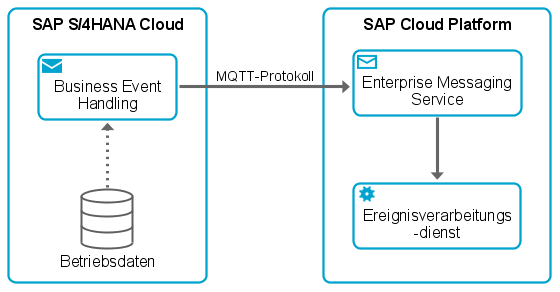
\includegraphics[width=.9\textwidth]{img/eventarch.png}	
    \caption[Softwarearchitektur des Ereignisverarbeitungsdienstes]
    {Softwarearchitektur des Ereignisverarbeitungsdienstes\protect\footnotemark}
    \label{fig:Softwarearchitektur des Ereignisverarbeitungsdienstes}
\end{figure}
\footnotetext{Eigene Darstellung}
\footnotetext{Die Abbildung dient lediglich der Visualisierung und ist nicht \ac{BPMN} 2.0 konform.}

% \subsection{Benutzung}

% \todo{mini process flow}

% \todo{JavaScript Coding hier platzieren}
